\documentclass[final]{cvpr}

% This version of CVPR template is provided by Ming-Ming Cheng.
% Please leave an issue if you found a bug:
% https://github.com/MCG-NKU/CVPR_Template.

% Copied baseplate from what Ishani Janveja did for our semantic noise cancelling paper last semester

%\documentclass[review]{cvpr}

\usepackage{times}
\usepackage{epsfig}
\usepackage{graphicx}
\usepackage{amsmath}
\usepackage{amssymb}
\usepackage{float}
\usepackage{graphicx}
\usepackage{caption}
\usepackage{float}
\usepackage{geometry}
\usepackage{graphbox}
\usepackage{subfig}
\usepackage{subcaption}
\usepackage{soul}
\usepackage{lipsum}
\usepackage{enumitem}
\usepackage{xcolor}
\usepackage{booktabs}
% Include other packages here, before hyperref.
\usepackage{algorithm}
\usepackage{algorithmic}
\usepackage[labelfont=bf]{caption}
% If you comment hyperref and then uncomment it, you should delete
% egpaper.aux before re-running latex.  (Or just hit 'q' on the first latex
% run, let it finish, and you should be clear).
\usepackage[pagebackref=true,breaklinks=true,colorlinks,bookmarks=false]{hyperref}


\def\cvprPaperID{****} % *** Enter the CVPR Paper ID here
\def\confYear{CVPR 2021}
%\setcounter{page}{4321} % For final version only
\newcommand{\es}[1]{\textcolor{red}{ES: #1}}

%%%%%%%%% TITLE
\title{Analysis of Zero-Agnostic Model for Copy Number Evolution} 

\author{
Sonali Merchia
}

\geometry{
 total={170mm,257mm},
 left=15mm,
 right=15mm,
 top=5mm,
}

\begin{document}

\twocolumn[{%
\renewcommand\twocolumn[1][]{#1}%
\maketitle
\thispagestyle{empty}
% \vspace{-18mm}


%
}]

\section{Introduction}

Reconstructing cancer phylogenies based on copy-number information is widely done using the copy-number transformation CNT model. This model splits up chromosomes into geographical regions called loci. It then represents a cell using a vector where each element represents a locus and the value represents the number of copies of that locus in the cell of interest. This vector is referred to as either a {\it copy number state\/} or {\it copy number profile}. The model then measures the distance between a pair of copy number profiles as the minimum number of mutations required to convert one state into the other~\cite{cnt_paper}. 

While useful and consistent with biological observations, there is no efficient algorithm using CNT to generate parsimonious cancer phylogenies due to its lack of symmetry. In {\it A zero-agnostic model for copy number evolution in cancer\/}~\cite{zcnt_paper}, a new model ZCNT is proposed that provides a mathematical simplification on the CNT model, allowing for an efficient algorithm to generate cancer phylogenies.

ZCNT allows for elements of the copy-number state to drop into the negatives and increase from zero to positive values. This is not possible in CNT because it would represent the spontaneous creation of a locus that did not exist previously or having a negative number of copies of DNA\@. This paper will analyze the ZCNT method to determine whether its findings are consistent with biology despite being based on a model inconsistent with biology. 

ZCNT supposedly closely mimics CNT distance but adds symmetry in an efficient manner. This paper will discuss the implications of using a symmetric property to mimic a non-symmetric property. 
% chktex-file 44
\section{Background}

\subsection{Cancer as an Evolutionary Process}

Cancer is an evolutionary process wherein cells grow and multiply irregularly due to genetic mutations. Mutations are when the DNA stored within cancer cells is altered in some way inconsistent with healthy somatic behavior. These mutations can take multiple different forms. Mutations are random and unique to each tumor but lead to the development of common hallmarks. These hallmarks are referred to as the ``Hallmarks of Cancer''~\cite{hallmarks_of_cancer} and are considered to be behaviors necessary for the cancer cells to grow and develop. 

\begin{figure}[ht]\label{fig:hallmarks}
    \centering
    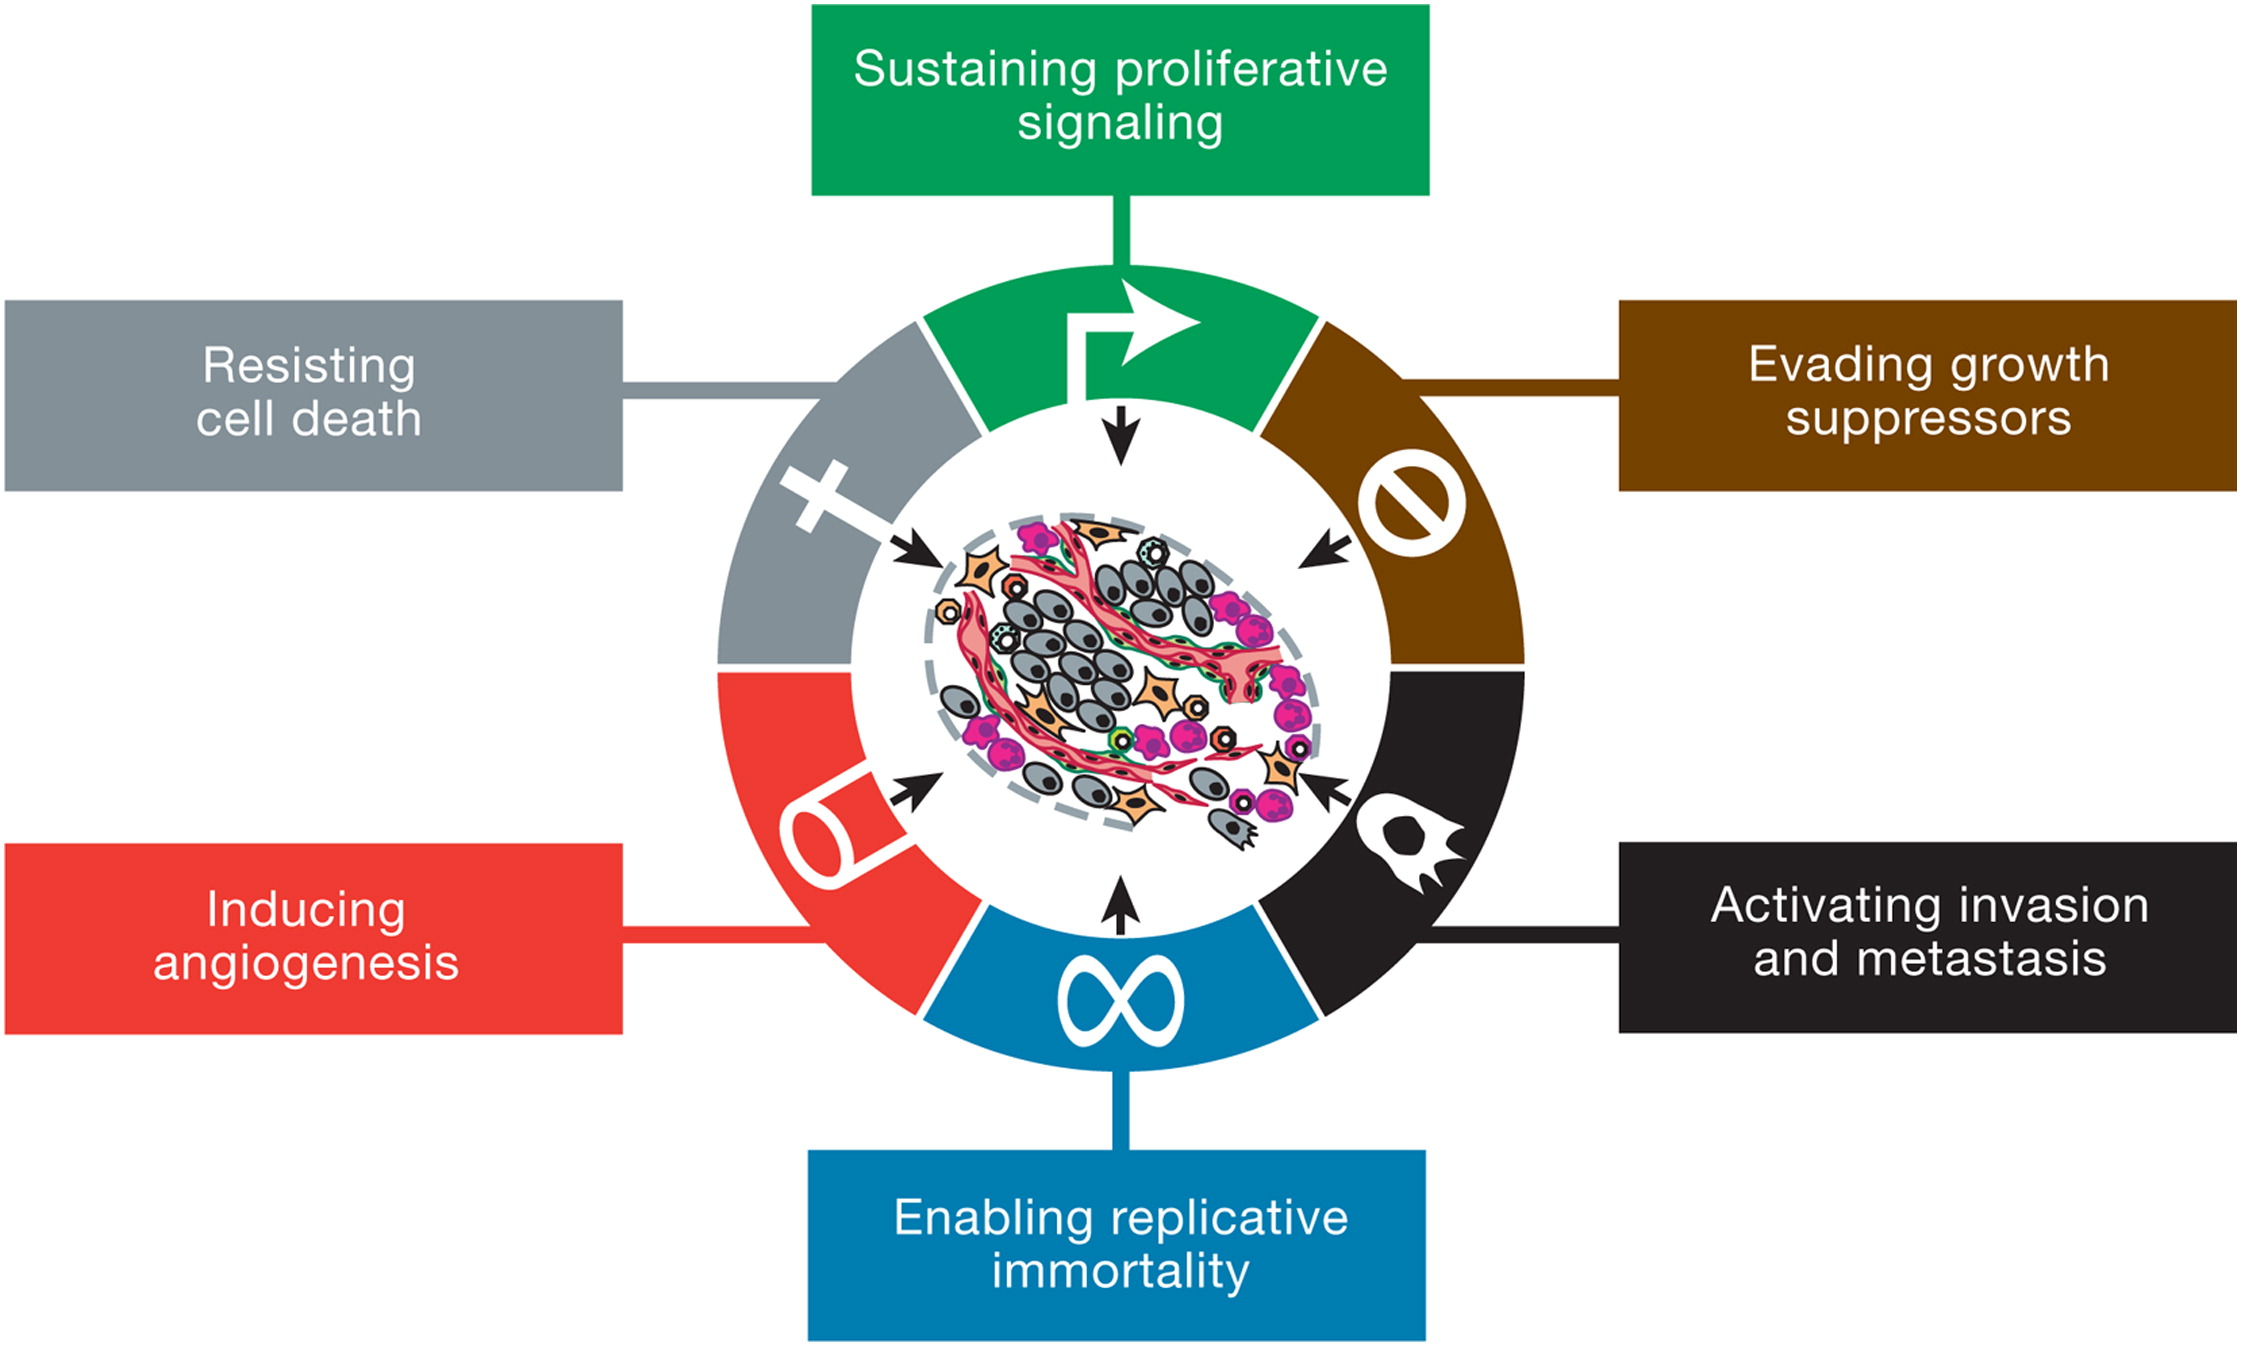
\includegraphics[width=0.45\textwidth]{figures/hallmarks.jpg}
    \caption{Hallmarks of Cancer~\cite{hallmarks_of_cancer}}
\end{figure}

Since these hallmarks are acquired through evolution, studying the phylogeneies of cancer cells can help inform how the cells acquired their abilities. Phylogenies are trees that trace the evolutionary history of a cell. In cancer phylogenics, trees are defined such that the nodes are ``clones''. Clones are defined as the genetic makeup of a population of cancer cells with common mutations. Studying cancer phylogenies can provide insight into tumor behaviors and open new avenues for potential treatments. 

\subsection{CNA-Based Phylogenies}

Different kinds of mutations affect the genome to different magnitudes. The most commonly studied kinds of mutations in cancer phylogenetics are Single Nucleotide Variants (SNVs) and Copy Number Aberrations (CNAs). SNVs are when a single base pair in the DNA is erroneously changed, inserted, or deleted. Meanwhile CNAs are when large geographical regions of base pairs are erroneously duplicated or deleted. 

\begin{figure}[ht]\label{fig:mutation_freq}
    \centering
    \includegraphics[width=0.45\textwidth]{figures/base_pair_mutations.png}
    \caption{Different kinds of mutations affect genomes differently and their affects are sometimes of vastly different scales. This graphic relates different kinds of mutations to the scale of base pairs affected by a mutation of that type.~\cite{lecture_2}}
\end{figure}

Researchers use genetic sequencing technologies to determine the state of SNVs and CNAs in a cell. The technology used determines what kind of analysis can be done with the data. If a technology has high coverage and low depth, it is considered optimal for deterimining SNVs in a cell. Meanwhile if a technology has low coverage and high depth, it is considered optimal for determining the copy number state of a cell. There are currently no high-throughput technologies that provide sufficient data to do both SNV and CNA analysis. Therefore most approaches are geared towards one or the other. The CNT and ZCNT models that are discussed in this paper will focus on CNAs. 

There are two main phylogenetic problems to be solved: the Large Parsimony Problem and the Small Parsimony Problem. Large Parsimony is when you are given the copy-number states of cells and aim to organize them into a rooted evolutionary tree wherein every cell has exactly one parent. Meanwhile Small Parsimony is when you are given the copy-number states of ``leaf-node'' cells and aim to generate the intermediary nodes of the phylogenetic tree. 

The core principle behind cancer phylogeny reconstruction is that mutations are rare~\cite{mutations_rare}. That means that in order to reconstruct cancer phylogeneies, it is useful to define distance functions representative of the number of mutations. These allow us to construct phylogenetic trees that would require few mutations to generate, encouraging parsimonious evolutionary trees. Both ZCNT and CNT define different algorithms to determine distance. 

\subsection{CNA-Based Distance Functions}

Both CNT and ZCNT models have mathematical definitions of events. In both models events represent a copy-number aberration that affects copy number profile $p$ over a range of loci from $s$ to $t$ inclusive ($s \leq t$) by increasing or decreasing the copy number by 1 (denoted by $b \in \{+1, -1\}$). 

They also both define the concept of a ``transformation'' to be a series of events. For instance, given events $(e_1, \hdots, e_n)$, a transformation would be defined as $T(p) = e_n(\hdots(e_1(p)))$. Both models define distance between two profiles to be the minimum number of events required to transform one profile into another ($\text{dist}(u, v) = \min_{T(u) = v} |T|$). Events in a transformation are communtative under ZCNT~\cite{zcnt_paper}.

\subsubsection{CNT}

\newcommand{\cnt}{\textbf{cnt}}
\newcommand{\zcnt}{\textbf{zcnt}}

{\bf Copy Number Event Formula}: ($c_{s, t, b}: \mathbb{Z}_+^n \rightarrow \mathbb{Z}_+^n$) 
\begin{equation}
    c_{s, t, b}{(p)}_i = \begin{cases}
        p_i + b & \text{if}~s \leq i \leq t~\text{and}~p_i \neq 0 \\ 
        p_i & otherwise
    \end{cases}
\end{equation}

Given two copy number profiles, it is not guaranteed that there will be a transformation from one to the other under the CNT model. For instance, given $u=[0,1]$ and $v=[1,0]$, $u$ would have to amplify a copy number from zero to one in order to transform into $v$. In these cases the distance is defined as $+\infty$. We will denote CNT distance between two profiles $u$ and $v$ as $\cnt(u, v)$.

Due to the lack of symmetry in the CNT model, two common methods have been employed to create symmetric measures from CNT for various parsimony algorithms.\vspace{5pt}

Both these algorithms are centered around getting the CNT distance in both directions. Mean Correction is when you take the average of the distances between two profiles. Median distance just takes the lower of the two distances.

\def\arraystretch{2}

\vspace{10pt}

\begin{tabular}{|c|c|}
    \hline
    {\bf Method} & {\bf Formula} \\  \hline \hline
    Mean Correction & $\frac{\cnt (u, v) + \cnt (v, u)}{2}$ \\ \hline
    Median Distance & $\min \{\cnt (u, v), \cnt (v, u)\}$ \\ \hline
\end{tabular}

\vspace{15pt}

Both of these definitions raise interesting questions about reachability. Mean correction amplifies unreachability because if either $\cnt(u, v)$ or $\cnt(v, u)$ does not exist, the mean correction will yield $+\infty$. Meanwhile median distance amplifies reachability because even if either $\cnt(u, v)$ or $\cnt(v, u)$ does not exist, median distance will yield a noninfinite number. 

Instead of using a distance with these constraints, it is common to use another kind of intermediary. Some papers use the {\it copy number triplet\/} (CN3) problem. Which aims to pick some intermediate profile $w$ that minimizes $\cnt(w, u) + \cnt (w, v)$~\cite{triplet_algorithm}. 

While CN3 provides symmetry, it comes at the cost of computational time. CNT distances can be computed in $O(n)$ time~\cite{linear_cnt} while the most optimal current algorithm for CN3 is $O(nB^7)$ where $B$ is the largest copy number in the input profiles~\cite{triplet_algorithm}. The benefit of using CN3 is that the value is symmetric and therefore works well with existing parsimony methods.

\subsubsection{ZCNT}

{\bf Zero-Agnostic Copy Number Event Formula} 

($c_{s, t, b}: \mathbb{Z}^n \rightarrow \mathbb{Z}^n$) 

\begin{equation}
    c_{s, t, b}{(p)}_i = \begin{cases}
        p_i + b & \text{if } s \leq i \leq t \\ 
        p_i & otherwise
    \end{cases}
\end{equation}

Notice that the only difference between the ZCNT and CNT model is the removal of the non-negativity constraint in the function signature and the condition to skip $p_i$ if $p_i$ is zero. We will denote ZCNT distance between two profiles $u$ and $v$ as $\zcnt(u, v)$. Unlike CNT distance, ZCNT distance always exists as a non-infinite number. 

In {\it A zero-agnostic model for copy number evolution in cancer\/}~\cite{zcnt_paper}, they propose the following closed-form formula for ZCNT distance: 

\begin{equation} \label{eq:1}
    \zcnt(u, v) = \frac{1}{2} ||\Delta (u) - \Delta (v)||_1
\end{equation}

where $\Delta (p)$ denotes another linear transform called {\it delta mapping\/} ($\Delta: \mathbb{Z}^{n} \rightarrow \mathbb{Z}^{n + 1}$)

\begin{equation} \label{eq:2}
    \Delta {(p)}_i = \begin{cases}
        p_1 - 2 & \text{if } i=1 \\ 
        2 - p_n & \text{else if } i=n+1 \\
        p_i - p_{i-1} & otherwise
    \end{cases}
\end{equation}

Due to ZCNT being the composition of two linear equations (Equations~\ref{eq:1} and~\ref{eq:2}), ZCNT can trivially be seen as an $O(n)$ algorithm. 
% chktex-file 8
\section{Proofs}

ZCNT is proposed as a distance metric~\cite{zcnt_paper}. In order to be a distance metric, ZCNT must satisfy the four following properties: 

\begin{enumerate}
    \item {\bf Identity:} $\zcnt (u, u) = 0$
    \item {\bf Positivity:} if $u \neq v$ then $0 < \zcnt (u, v)$
    \item {\bf Symmetry:} $\zcnt (u, v) = \zcnt (v, u)$
    \item {\bf Triangularity:} $\zcnt (u, v) \leq \zcnt (u, w) + \zcnt (w, v)$
\end{enumerate}

Below we will prove each of these properties mathematically. 

\subsection{Identity}

The identity property can be mathematically obtained without any additional lemmas. 

\begin{theorem}
    Let $u$ be some arbitrary copy-number profile under the ZCNT model. 
    
    Then $\zcnt (u, u) = 0$
\end{theorem}

\noindent {\bf Proof:}
\begin{align*}
    \textbf{Statement} & & \textbf{Explanation} \\
    \cline{1-3}
    \zcnt (u, u) &= \frac{1}{2} || \Delta(u) - \Delta(u) ||_1  & \text{Equation~\ref{eq:1}}\\ 
    &= \frac{1}{2} || \mathbf 0 ||_1 &\text{Subtract}\\ 
    &= \frac{1}{2} (0) &\text{Simplify} \\ 
    \zcnt (u, u) &= 0 &\text{Simplify}
\end{align*}

\subsection{Positivity}

\begin{theorem}
    Let $u$ and $v$ be some arbitrary copy-number profiles under the ZCNT model. 
    
    Then $u \neq v \implies 0 < \zcnt (u, v)$.
\end{theorem}


\noindent {\bf Proof:}

The proof of positivity is based on the principle that the L1 norm is a distance metric. Therefore by the positivity property, the L1 norm of any nonzero vector will be greater than $0$. We can write this formally as:
\begin{lemma}\label{lemma:l1_positivity}
    Let $u$ and $v$ be some arbitrary vector in $\mathbb{R}^n$. 
    
    Then $u \neq v \implies 0 < ||u - v||_1$.
\end{lemma}

Since $\Delta$ is a bijective function~\cite{zcnt_paper}, we know that every input has a unique output. We also know that every output has a unique input. Therefore if $u \neq v$, then the delta mappings will be different. We can write this formally as: 

\begin{lemma}\label{lemma:delta_bijection}
    Let $u$ and $v$ be some copy number profiles under the ZCNT model. Let $\Delta(\cdot)$ be the function to convert a copy number profile to its respective delta mapping. 
    
    Then $u \neq v \iff \Delta(u) \neq \Delta(v)$
\end{lemma}

Using these properties, we can write the following proof for the positivity property of ZCNT

\begin{align*}
    \textbf{Statement} & & \textbf{Explanation} \\
    \cline{1-3} \\
    u \neq v &\implies \Delta(u) \neq \Delta(v) & \text{Lemma}~\ref{lemma:delta_bijection} \\ 
    & \implies \Delta(u) - \Delta(v) \neq 0 & \text{Subtraction}\\
    & \implies 0 < ||\Delta(u) - \Delta(v)||_1 & \text{Lemma}~\ref{lemma:l1_positivity} \\
    & \implies 0 < \frac{1}{2}||\Delta(u) - \Delta(v)||_1 & \text{Multiply} \\
    u \neq v & \implies 0 < \zcnt (u, v) & \text{Equation}~\ref{eq:1}
\end{align*}

\subsection{Symmetry}
\begin{theorem}
    Let $u$ and $v$ be some arbitrary copy-number profiles under the ZCNT model. 
    
    Then $\zcnt (u, v) = \zcnt (v, u)$
\end{theorem}

\noindent {\bf Proof:}

\begin{corollary}\label{corollary:abs_val}
    $\forall x \in \mathbb{R}$, $|x| = |-x|$ by absolute value definition
\end{corollary}

\begin{align*}
    \textbf{Statement} & & \textbf{Explanation} \\
    \cline{1-3} \\
    \zcnt (u, v) &= \frac{1}{2} || \Delta(u) - \Delta(v) ||_1 & \text{Equation}~\ref{eq:1} \\ 
    &= \frac{1}{2} || -(\Delta(u) - \Delta(v)) ||_1 & \text{Corollary}~\ref{corollary:abs_val} \\
    &= \frac{1}{2} ||  \Delta(v) - \Delta(u) ||_1 & \text{Multiply}\\ 
    \zcnt (u, v) &= \zcnt(v, u) & \text{Equation}~\ref{eq:1}
\end{align*}

\subsection{Triangularity} 

\begin{theorem}
    Let $u$ and $v$ be some arbitrary copy number profiles under the ZCNT model. 

    Then for all copy number profiles $w$, 
    
    $\zcnt (u, v) \leq \zcnt (u, w) + \zcnt (w, v)$
\end{theorem}

\noindent {\bf Proof:}

Let $\mathbf x = (\Delta(u) - \Delta(w))$ and $\mathbf y = (\Delta(w) - \Delta(v))$. From this we get: 

\begin{alignb}\label{eq:substitutions}
    ||\mathbf{x}||_1 &= ||\Delta(u) - \Delta(w)||_1 \\ 
    &=2 \times\zcnt(u, w) \\
    ||\mathbf{y}||_1 &= ||\Delta(w) - \Delta(v)||_1 \\ 
    &=2 \times\zcnt(w, v) \\
    ||\mathbf{x} + \mathbf{y}||_1 &= ||\Delta(u) - \Delta(w) + \Delta(w) - \Delta(v)||_1 \\ 
    &= ||\Delta(u) - \Delta(v)||_1 \\ 
    &= 2 \times\zcnt(u, v)
\end{alignb} 

Since L1 is a distance metric we can write its triangularity property formally as follows: 

\begin{lemma}\label{lemma:l1_triangular}
    $\forall x, y \in \mathbb{R}^n, ||\mathbf x + \mathbf y||_1 \leq ||\mathbf x||_1 + ||\mathbf y||_1$
\end{lemma}

Using these two equations, we can formally prove the triangularity property of ZCNT as follows: 

\begin{align*}
    \textbf{Statement} & & \textbf{Explanation} \\
    \cline{1-3} \\
    ||\mathbf x + \mathbf y||_1 & \leq ||\mathbf x||_1 + ||\mathbf y||_1 & \text{Lemma}~\ref{lemma:lemma:l1_triangular} \\ 
    2 \times \zcnt(u, v) & \leq 2[\zcnt(u, w) + \zcnt(w, v)] & \text{Substitutions~\ref{eq:substitutions}} \\ 
    \zcnt(u, v) &\leq \zcnt(u, w) + \zcnt(w, v) & \text{Divide}
\end{align*}
\section{Methods}
Since ZCNT is a metric that is meant to emulate CNT, the question of behavior across symmetry exists. CNT is not a symmetric property and doesn't always exist. If ZCNT typically approximates CNT, how does it behave when the corresponding CNT distance does not exist? Does it trend towards $+\infty$ when $\cnt(u, v) = \infty$ or is there another behavior?

\vspace{10pt}

\noindent The points of interest in this paper are: 

\begin{enumerate}\label{enumerate:questions}
    \item How well does ZCNT replicate CNT\@? How well does it replicate CN3?
    \item How does ZCNT behave when the corresponding CNT does not exist?
    \item How often do reachability issues show up in simulated data? 
    \item How often do reachability issues show up in real data? 
    \item Does ZCNT more closesly mimic Median Distance or Mean Correction?
\end{enumerate}

\subsection{Comparing ZCNT and CNT}\label{section:comp_dist}

In order to compare ZCNT and CNT distances, pairwise distances were generated for simulated data. The data was the same simulated data from the original ZCNT paper~\cite{zcnt_paper}. There were three kinds of distances generated for every simulation pair: ZCNT, CNT, and CN3. 

The distances were filtered so we only considered the distances where CNT for that pairing was not $+\infty$. Since both ZCNT and CN3 always exist at a noninfinite value, this was the only filter. Then the relative error was calculated for each distance pairing (all combinations of ZCNT, CNT, and CN3). 

\subsection{Behavior of ZCNT when CNT is infinite}\label{section:behavior}

In order to determine ZCNT behavior when CNT is infinite, the same simulated distances in Section~\ref{section:comp_dist} were used to classify copy-number pairings into three classes: 


{\bf Class 1:} $\cnt(u, v)$ and $\cnt(v, u)$ both exist

{\bf Class 2:} $\cnt(u, v)$ exists but $\cnt(v, u)$ does not 

{\bf Class 3:} Neither $\cnt(u, v)$ nor $\cnt(v, u)$ exist 

Then an analysis was done based on the distribution of the corresponding ZCNT distances. 


\subsection{Reachability in Simulated Data}\label{section:simulated_reachability}
The same simulated data from the prior two sections was put through Lazac, a ZCNT Large Parsimony algorithm~\cite{zcnt_paper}. Then, using the calculated pairwise distances in CNT and ZCNT, two statistics were taken: 

\begin{enumerate}
    \item The percentage of edges in the overall tree represent biologically infeasible transformations.
    \item The percentage of ancestor-descendant relationships that were biologically infeasible.
\end{enumerate}

We define ``biologically infeasible'' transformations to be transformations wherein a copy-number goes from zero to a positive number. These can easily be determined by calculating the CNT distances. If the CNT distance between two nodes is $\infty$, the transformation is biologically infeasible. 

For ancestor-descendant relationships between an ancestor $u$ and a descendant $v$, the pairing is considered illegal if and only if an edge drawn straight between them would be biologically infeasible.

\subsection{Reachability in Real Data}\label{section:real_reachability}
In order to determine how often reachability issues show up in real data, the same classification process described in Section~\ref{section:behavior} will be performed on real and simulated data. Bar graphs will be constructed to see if real data has a different class distribution than simulated data. 

\subsection{ZCNT Against Symmetric CNT Distances}\label{section:symmetric_cnt_vs_zcnt}
In order to determine ZCNT's behavior against symmetric CNT measures like Median Distance or Mean Correction, ZCNT and CNT distances will be calculated for simulated data. Then the error between ZCNT and the different symmetric CNT measurements will be calculated and compared. 

In order for figures to be legible, cases where the symmetric measures equal $\infty$ will be excluded. To make sure that the data is still represented, the number of ommitted values will be included for each distance measure.

% chktex-file 44
\section{Results}

\subsection{Comparing ZCNT and CNT}\label{section:comp_dist_res}

\begin{figure}[ht]
    \centering
    \includegraphics[width=0.45\textwidth]{figures/dist_fig_hist.png}
    \caption{Relative error for the pairwise-distances of CNT, CN3, and ZCNT methods on simulated data as described in Section~\ref{section:comp_dist}. This includes error from multiple test suites where the number of cells was 200 and the loci were from \{1000, 2000, 3000, 4000\}. The graph was then normalized so that the area under the curve for each comparision class would equal 1. Pairings where the corresponding CNT distance was $\infty$ were excluded from the graph.}\label{fig:dist_figure_histogram}
\end{figure}

\begin{figure}[ht]
    \centering
    \includegraphics[width=0.45\textwidth]{figures/dist_fig_boxplot.png}
    \caption{Relative error for the pairwise-distances of CNT, CN3, and ZCNT methods on simulated data as described in Section~\ref{section:comp_dist}. Note that outliers are removed from this plot. This includes error from multiple test suites where the number of cells was 200 and the loci were from \{1000, 2000, 3000, 4000\}. Pairings where the corresponding CNT distance was $\infty$ were excluded from the graph.}\label{fig:dist_fig_box}
\end{figure}

\begin{figure}[ht]
    \centering 
    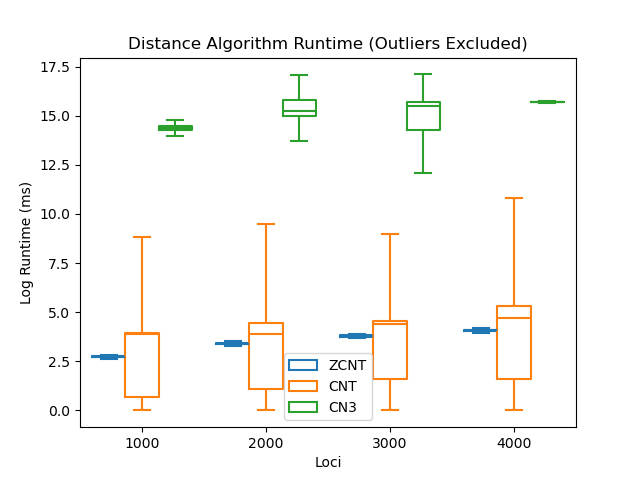
\includegraphics[width=0.45\textwidth]{figures/time_fig.png}
    \caption{This shows the running times of running the different distance methods on different numbers of loci on a logorithmic scale. All trials used 200 cells. This was computed using simulated data. The number of loci were from \{1000, 2000, 3000, 4000\}.}\label{fig:time_fig}
\end{figure} 

The results for the methods described in Section~\ref{section:comp_dist} to compare the three distance algorithms ZCNT, CNT, and CN3 are shown in Figures~\ref{fig:dist_figure_histogram} and~\ref{fig:dist_fig_box} include five suites with a constant number of 200 cells and varying numbers of loci. Most other analyses also compare across varying number of cells and random seeds. This analysis does not do so due to the running time involved in calculating CN3 distances. A figure demonstrating this running time is included as Figure~\ref{fig:time_fig}. This significantly higher runtime was expected due to CN3 being an $O(nB^7)$ algorithm while ZCNT and CNT are both linear time $O(n)$ algorithms. 

Figures~\ref{fig:dist_figure_histogram} and~\ref{fig:dist_fig_box} show that ZCNT and CN3 have more in common than any other pairing. However the relative error for the grand majority of the comparision classes falls below $10\%$. Interestingly, even the most different pairing (ZCNT and CNT) mostly had error falling below $20\%$. 

\begin{figure}[ht]
    \centering
    \includegraphics[width=0.45\textwidth]{figures/classes_hist.png}
    \caption{Absolute value of pairwise distances generated with ZCNT according to Section~\ref{section:behavior}. Class 1 is composed of ZCNT distances $\zcnt(u, v)$ where $\cnt(u, v) \neq \infty$ and $\cnt(v, u) \neq \infty$. Class 2 is composed of ZCNT distances $\zcnt(u, v)$ where exactly one of $\cnt(u, v)$ and $\cnt(v, u)$ equals $\infty$. Class 3 is composed of ZCNT distances where $\cnt(u, v) = \cnt(v, u) = \infty$. The distances are from simulated data where the number of cells were in \{200 300 400 500 600 1200\} and the number of loci were from \{1000, 2000, 3000, 4000\} across seven random seeds. The data was then binned and normalized so the area under each curve is 1.}\label{fig:classes_hist}
\end{figure}

\begin{figure}[ht]
    \centering
    \includegraphics[width=0.45\textwidth]{figures/classes_box.png}
    \caption{Absolute value of pairwise distances generated with ZCNT according to Section~\ref{section:behavior}. Note that outliers are removed from this plot. Class 1 is composed of ZCNT distances $\zcnt(u, v)$ where $\cnt(u, v) \neq \infty$ and $\cnt(v, u) \neq \infty$. Class 2 is composed of ZCNT distances $\zcnt(u, v)$ where exactly one of $\cnt(u, v)$ and $\cnt(v, u)$ equals $\infty$. Class 3 is composed of ZCNT distances where $\cnt(u, v) = \cnt(v, u) = \infty$. The distances are from simulated data where the number of cells were in \{200 300 400 500 600 1200\} and the number of loci were from \{1000, 2000, 3000, 4000\} across seven random seeds.}\label{fig:classes_box}
\end{figure}

\subsection{Behavior of ZCNT when CNT is infinite}\label{section:behavior_res}

Figures~\ref{fig:classes_hist} and~\ref{fig:classes_box} show the results from the methodology described in Section~\ref{section:behavior}. The three classes seem to all follow fairly normal distributions. Class 1 has the lowest mean while class 3 has the highest mean. This seems to signify to that reachability in CNT corresponds to lower ZCNT values. This is good because if trees minimize distance, they will also likely favor pairings in Class 1 over all other classes and favor pairings in Class 2 over pairings in Class 3. This behavior would align with biologically feasible transitions. 

\subsection{Reachability in Simulated Data}\label{section:simulated_reachability_res}

Figures~\ref{fig:illegal_desc} and~\ref{fig:illegal_edges} show the results from the methodology described in Section~\ref{section:simulated_reachability}. These show that as the number of loci increases, biologically infeasible edges become less common. The number of cells involved in the phylogeny appears to decrease the spread of the data, but not shift it. It also shows that biologically infeasible edges are relatively rare, with 22 out of 168 trees (13.09\%) having no illegal edges or ancestor-descendant relationships. The rate of illegal edges is very infrequent with is very small. Even the tree with the most illegal edges has at most 7.36\% of illegal edges. 

\begin{figure}[ht]
    \centering
    \includegraphics[width=0.45\textwidth]{figures/illegal_desc.png} 
    \caption{The percentage of overall ancestor-descendant pairs in Lazac-produced trees on simulated data where it would be biologically infeasible for the descendant to be produced from the ancestor. The number of cells were in \{200 300 400 500 600 1200\} and the number of loci were from \{1000, 2000, 3000, 4000\} across seven random seeds.}\label{fig:illegal_desc}
\end{figure}

\begin{figure}[ht]
    \centering
    \includegraphics[width=0.45\textwidth]{figures/illegal_edges.png}
    \caption{The percentage of overall edges in Lazac-produced trees on simulated data where it would be biologically infeasible for the child to be produced from the parent. The number of cells were in \{200 300 400 500 600 1200\} and the number of loci were from \{1000, 2000, 3000, 4000\} across seven random seeds.}\label{fig:illegal_edges}
\end{figure}

\begin{figure}[ht]
    \centering
    \includegraphics[width=0.45\textwidth]{figures/cumulative_plot.png}
    \caption{This shows a cumulative plot that shows what percentage of simulated trees contain biologically infeasible edges or ancestor-descendent relationships. The number of cells were in \{200 300 400 500 600 1200\} and the number of loci were from \{1000, 2000, 3000, 4000\} across seven random seeds.}\label{fig:cumulative_trees}
\end{figure}

Figure~\ref{fig:cumulative_trees} shows the cumulative rate of illegal edges or ancestor-descendant relationships. Illegal edges are the source of illegal ancestor-descendant relationships so the ancestor-descendant curve is just a horizontally stretched version of the illegal edges curve. The amount of stretch shows how many cells are descended from illegal edges. 

The plot shows that more than half the trees have fewer than 2.5\% illegal edges. The trees with the fewest illegal edges don't appear to have many descendants of those illegal relationships as shown by the curves matching for the first portion of the graph. This implies that for those trees, the ZCNT model predicts decently biologically feasible trees. However for roughly 40\% of the trees, an increasing proportion of nodes are descended from impossible transitions like zero-amplifications. 

\subsection{Reachability in Real Data}\label{section:real_reachability_res}

\begin{figure}[ht]
    \centering 
    \includegraphics[width=0.45\textwidth]{figures/classes_real_bar.png}
    \caption{The frequency distribution of classes described in Section~\ref{section:behavior} using real data. The real data is from patient 8 of the study on metastatic prostate cancer~\cite{real_data}. The data measures across 10 cells, a maximum of 22 chromosomes per cell, and a maximum of 38 loci per chromosome. Pairwise CNT distances were generated for each cell. Then each pairing was classified as follows. Class 1 is composed of pairings where $\cnt(u, v) \neq \infty$ and $\cnt(v, u) \neq \infty$. Class 2 is composed of pairings where exactly one of $\cnt(u, v)$ and $\cnt(v, u)$ equals $\infty$. Class 3 is composed of pairings where $\cnt(u, v) = \cnt(v, u) = \infty$.}\label{fig:classes_real_bar}
\end{figure}

\begin{figure}[ht]
    \centering 
    \includegraphics[width=0.45\textwidth]{figures/classes_sim_bar.png}
    \caption{The frequency distribution of classes described in Section~\ref{section:behavior} using simulated data. The simulated data was generated such that the number of cells were in \{200 300 400 500 600 1200\} and the number of loci were from \{1000, 2000, 3000, 4000\} across seven random seeds. Pairwise CNT distances were generated for each suite and then classified as follows. Class 1 is composed of pairings where $\cnt(u, v) \neq \infty$ and $\cnt(v, u) \neq \infty$. Class 2 is composed of pairings where exactly one of $\cnt(u, v)$ and $\cnt(v, u)$ equals $\infty$. Class 3 is composed of pairings where $\cnt(u, v) = \cnt(v, u) = \infty$.}\label{fig:classes_sim_bar}
\end{figure}

Figures~\ref{fig:classes_real_bar} and~\ref{fig:classes_sim_bar} show the results from the methods described in Section~\ref{section:real_reachability}. They show that the number of pairings falling into Classes 1 and 3 are about equal in real data but the simulated data shows a preference for Class 1. 

For both kinds of data, the frequency of pairings falling into Class 2 is the highest but the peak is stronger in the real data. This could be due to a number of factors including the fact that there is significantly less data available for the real data compared to the simulated data. 

\subsection{ZCNT Against Symmetric CNT Distances}\label{section:symmetric_cnt_vs_zcnt_res}

\begin{figure}[ht]
    \centering 
    \includegraphics[width=0.45\textwidth]{figures/sym_fig_hist.png}
    \caption{The relative error of ZCNT against CNT measures that correct for symmetry (Median Distance and Mean Correction) on simulated data as described in Section~\ref{section:symmetric_cnt_vs_zcnt}. The distances are from simulated data where the number of cells were in {200 300 400 500 600 1200} and the number of loci were from {1000, 2000, 3000, 4000} across seven random seeds. Pairwise ZCNT and CNT distances were generated for all cells in the data. Then Mean Correction and Median Distance were calculated for all CNT distances. Pairings where the relative distance would be $\infty$ due to Mean Correction or Median Distance being $\infty$ were excluded.}\label{fig:symmetric_rel_err_hist}
\end{figure}

\begin{figure}[ht]
    \centering
    \includegraphics[width=0.45\textwidth]{figures/sym_fig_boxplot.png}
    \caption{The relative error of ZCNT against CNT measures that correct for symmetry (Median Distance and Mean Correction) on simulated data as described in Section~\ref{section:symmetric_cnt_vs_zcnt}. Note that outliers are excluded from the graph. The distances are from simulated data where the number of cells were in {200 300 400 500 600 1200} and the number of loci were from {1000, 2000, 3000, 4000} across seven random seeds. Pairwise ZCNT and CNT distances were generated for all cells in the data. Then Mean Correction and Median Distance were calculated for all CNT distances. Pairings where the relative distance would be $\infty$ due to Mean Correction or Median Distance being $\infty$ were excluded.}\label{fig:symmetric_rel_err_box}
\end{figure}

\begin{figure}[ht]
    \centering 
    \begin{tabular}{|c|c|c|c|} \hline
        Loci & Mean Correction & Median Distance & Total \\ \hline \hline
        1000 & 76.57\% & 27.67\% & 52.12\% \\ 
        2000 & 76.06\% & 29.34\% & 52.70\% \\ 
        3000 & 51.22\% & 8.91\% & 30.07\% \\ 
        4000 & 44.51\% & 5.88\% & 25.19\% \\ \hline
        Total & 62.09\% & 17.95\% & 40.02\% \\ \hline
    \end{tabular}
    \caption{The percentage of pairwise distances excluded from plots in Figures~\ref{fig:symmetric_rel_err_hist} and~\ref{fig:symmetric_rel_err_box} due to the value being $\infty$ rounded to the nearest hundredth of a percent.}\label{fig:excluded_table}
\end{figure}
    
Figures~\ref{fig:symmetric_rel_err_hist} and~\ref{fig:symmetric_rel_err_box} show the results of the methods described in Section~\ref{section:symmetric_cnt_vs_zcnt}. Figure~\ref{fig:symmetric_rel_err_hist} shows that ZCNT's relative error with Mean Correction and with Median Distance are near identical. Figure~\ref{fig:symmetric_rel_err_box} shows that the number of loci in the sample does not strongly affect the relative error between ZCNT and central CNT measurements. 

Figure~\ref{fig:excluded_table} shows what percentage of pairs were excluded for each kind of distance measurement. Since ZCNT always exists as a noninfinite value, this is a representation of how often Mean Correction and Median Distance came up with infinite values. It seems that the more loci there are, the smaller percentage of pairings result in infinite values regardless of the approach. This is interesting because the number of loci does not affect relative error. This means that the excluded values due to infinte Median Distance or Mean Correction values do not strongly affect the distribution of the distances.

The percentage of pairings resulting in infinite values is substantially higher for Mean Correction than it is for Median Distance. This is to be expected because for any distance from profile $u$ to $v$, both $\cnt(u, v)$ and $\cnt(v, u)$ must be noninfinite for the Mean Correction to be noninfinite. Meanwhile for Median Distance, only one of them must be noninfinite for the resulting value to be noninfinite.
\section{Discussion}

Despite the basis of ZCNT being a biologically inaccurate phenomenon, the results from using this approach seem produce more biologically accurate results. Results from this paper show that biologically impossible phenomena like zero-amplification are improbable in ZCNT-Based Models. 

This paper's research questions (See list~\ref{enumerate:questions}) are answered by our analyses as follows:

\begin{enumerate}
    \item The analysis presented in Section~\ref{section:comp_dist_res} shows that ZCNT closesly replicates both CN3 and CNT distance measurements. However it appears to more closely mimic CN3 distance than CNT distance. This is perhaps due to the shared symmetric nature of ZCNT and CN3 algorithms. 
    \item The analysis presented in Section~\ref{section:behavior_res} shows that ZCNT trends lower when the corresponding CNT exists in both directions, marginally higher when unreachable in one directon, and marginally higher still if unreachable in both directions. 
    \item The analysis presented in Section~\ref{section:simulated_reachability_res} shows that the more data points available, the more biologically feasible the results from ZCNT Large Parsimony trees will be. More loci means that the number of illegal edges and ancestor-descendant relationships will decrease. This is perhaps because more loci increases the spread of the ZCNT distance, decreasing the average cost per edge and causing a stronger preference for easily reachable profiles. More analysis could be done in this avenue to determine if this is the case. 
    \item The analysis presented in Section~\ref{section:real_reachability_res} shows that the reachability distributions in real data are roughly the same as the reachability distributions in simulated data. The difference appears to be in the spread of the reachability with real data having a larger difference in frequency. More analysis could be done in this avenue to see if these differences are present when run on a larger collection of real data. 
    \item The analysis presented in Section~\ref{section:symmetric_cnt_vs_zcnt_res} shows that ZCNT adheres to Median Distance and Mean Correction approximately the same amount regardless of how many values either measure deems to be infinite. 
\end{enumerate}


\section{Conclusion}

{
\small
\bibliographystyle{ieee_fullname}
\bibliography{ref_manual}
}

\end{document}


